\section{Opis implementacji}
Aplikacja została napisana przy użyciu języków programowania bazujących na maszynie wirtualnej javy:
\begin{enumerate}
  \item Kotlin - podstawowy język użtyty do implementacji (prawie 90\% projektu)
  \item Java 8 - język użyty do generowania statystyk wykonania algorytmów
  \item JavaFX - technologia zastosowana do stworzenia graficzego interfejsu użytkownika (wraz z CSS)
\end{enumerate}

Architektura aplikacji jest modułowa. Zostały wydzielone części odpowiedzialne za obliczenia matematyczne, implementacje algorytmów, zapis i odczyt plików CSV, generację statystyk, definicję modelu danych oraz moduł zawierający aplikację korzystająca z pozostałych pakietów (\hyperref[fig:arch]{rys.~\ref*{fig:arch}}).

\begin{figure}[h]
  \center
  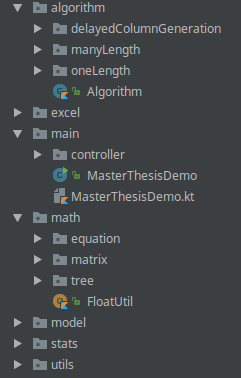
\includegraphics[scale=0.7]{../image/arch.png}
  \caption{Architektura aplikacji}
  \label{fig:arch}
\end{figure}

Architektura modułu odpowiedzialnego za implementację algorytmów posiada strukturę wzorca projektowego fasada. Klasy odpowiedzialne za konkretną implementację metody obliczenia rozkrojów rozszerzają klasę abstarkacyjną która definiuje wspólne funkcje oraz deklaruje metody które powinny zostać zdefiniowane w klasach potomnych. Główny moduł aplikacji wraz z modułem odpowiedizlanym za model danych tworzy implementację wzoraca Model-Widok-Kontroler (MVC). Klasa kontrolera zarządza widokiem stworzonym w języku FXML.

Rysunki \ref{fig:empty_win} oraz \ref{fig:fill_win} przedstawiają okno aplikacji, odpowiednio przed wypełnieniem danymi oraz po zakończeniu obliczeń.

\begin{figure}[h]
  \center
  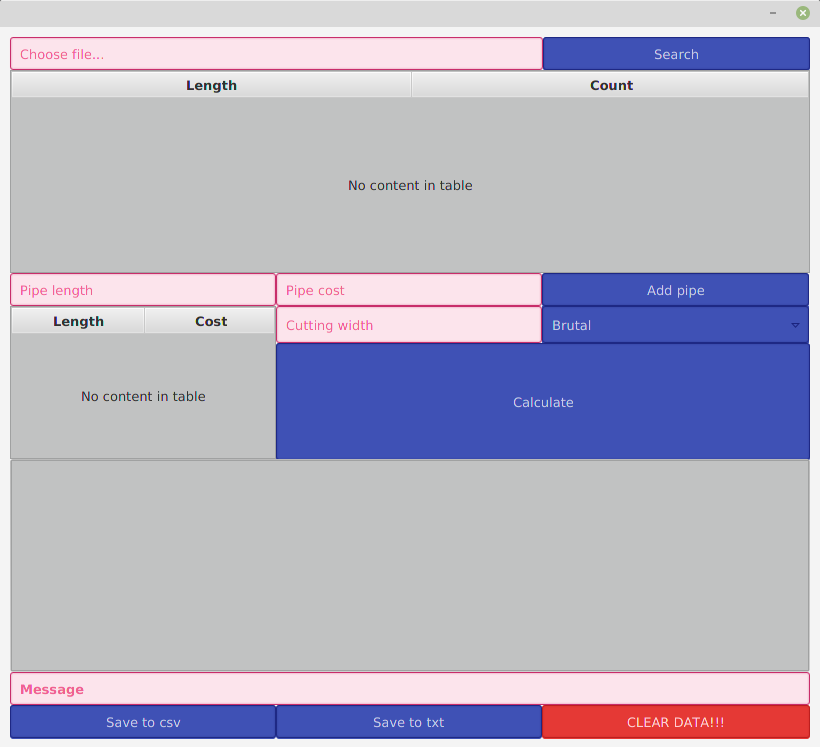
\includegraphics[scale=0.4]{../image/empty_win.png}
  \caption{Początkowe okno aplikacji}
  \label{fig:empty_win}
\end{figure}

\begin{figure}[h]
  \center
  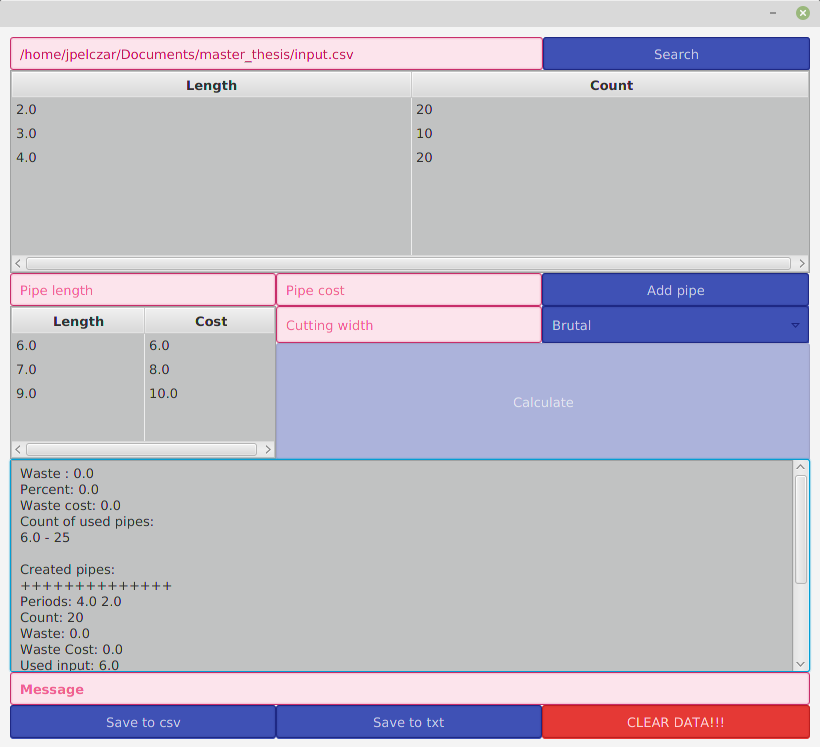
\includegraphics[scale=0.4]{../image/fill_win.png}
  \caption{Aplikacja po zakończonych obliczeniach}
  \label{fig:fill_win}
\end{figure}

Program posiada możliwość wczytania danych z pliku CSV, a następnie zapisanie danych wyjściowych również do pliku CSV lub TXT. Kolejnymi zaimplementowanymi funkcjonalnościami są:
\begin{enumerate}
  \item wyświetlenie danych wejściowych w oknie aplikacji
  \item wybór algorytmu rozkroju
  \item dodanie wielu długości podstawowych z różnym kosztem - domyślnie koszt jest równy długości.
  \item wyświetlenie długości podstawowych w oknie aplikacji
  \item dodanie szerkości cięcia dla metody brutalnej siły
  \item wyświetlenie wyniku w oknie aplikacji
\end{enumerate}

\subsection{Java}
Język programowania Java jest jezykiem obiektowym z elementami programowania funkcyjnego wprowadzonymi od wersji 8. Aplikacje stworzone w tej technologii mogą być stosowane w różnych systemach operacyjnych, gdyż programy napisane w języku Java są kompilowane do plików class które umieszczane są w skompresowanej paczce jar. Pliki class następnie są przetwarzane przez maszynę wirtualną Javy (JVM - Java Virtual Machine) do postaci bytecode który jest wykonywany na urządzeniu. Istnieją implementacje JVM na większość używanych platform.

Tworzenie aplikacji w technologii Java jest możliwe poprzez użycie zestawu JDK (Java Development Kit). Uruchamianie tych aplikacji jest możliwe w środowisku JRE (Java Runtime Environment)  (\hyperref[fig:java_arch]{rys.~\ref*{fig:java_arch}}).

\begin{figure}[h]
  \center
  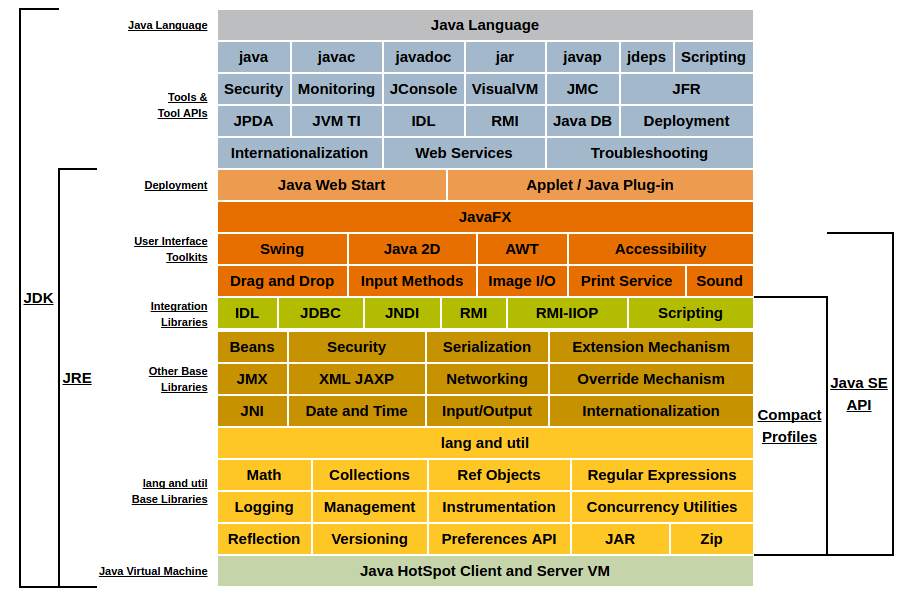
\includegraphics[scale=0.4]{../image/java_arch.png}
  \caption{Elementy składowe technologi Java \cite{OracleJavaArch}}
  \label{fig:java_arch}
\end{figure}

Podstawowym elementem technologii jest maszyna wirtualna. Jest to element technologii odpowiedzialny za niezależność programów od specyfikacji urządzenia oraz systemu operacyjnego. JVM jest abstarakcyjną maszyną obliczeniową. Podobnie jak rzeczywiste urządzenia posiada zestaw instrukcji pozwlających na sterowanie nią oraz wyonywanymi zadaniami. Maszyna wirtualna Javy nie zna języka Java, jedynie jego postać binarną zapisana w plikach class. Pliki te zawierają instrukcje dla JVM lub bytecode oraz inne wymagane informacje. Wiele języków programowania wykorzystuje tą cechę maszyny wirtualnej. Wymaganiem jest aby program był w postaci poprawnego pliku class, aby mógł zostać wykonany na maszynie wirtualniej.

Technologia Java zawiera ponadto zestaw podstawowaych bibliotek pozwlających między innymi na budowanie plików JAR, refleksję czyli dostęp do metod oraz pól klasy bez zachowania zasad bezpieczeństwa, zdalne wywoływanie metod (RMI) oraz tworzenie graficznego interfejsu użytkownika Swing oraz AWT. Środowisko deweloperskie jest rozszerzone o narzędzia potrzebne do stworzenia programu, przykładowo: javac - kompilator przetwarzający pliki java do plików class, javadoc - narzędzie do tworzenia dokumentacji oraz język opisu interfejsów IDL służacy do komunikacji międzyprocesowej.
\subsection{Kotlin}
Kotlin jest obiektowym językiem programowania który jest interpretowany do bytecode wywoływanego na maszynie wirtualnej Javy. Kotlin w porównaniu z Javą wnosi usprawnienia do programownaia proceduralnego. Kotlin jest zgodny z językiem Java, odnosi to skutek w możliwości łączenia obu języków programowania. Jest to technologia podobna do języka Scala jednak czas kompilacji został skrócony. Jest to język silnie rozwijający się w środowisku programistycznym Androida. Dopiero najnowsza wersja narzędzi deweloperskich Androida pozwala na wykorzystywanie niektórych elementów Javy 8. Kotlin zmniejsza liczbę nadmiarowego kodu potrzebnego do napisania przez programistę. Głównymi celami stworzenia technologii Kotlin były: pełna kompatybilność z językiem Java, zwiększenia bezpieczeństwa względem Javy (null safe), bardziej elastyczny oraz nieskomplikowany kod. Jedną z najciekawszych funkcjonalności języka Kotlin jest tworzenie metod rozszerzających daną klasę. Przykładowo może zostać zdefiniowana metoda $isNotEmpty()$ dla klasy $String$:
\lstset{language=Java}
\begin{lstlisting}[frame=single]
  fun String.isNotEmpty() = !this.isEmpty()
\end{lstlisting}
Metoda ta będzię dostępna dla każdego obiektu typu $String$ w programie.
\subsection{JavaFX}
